\capitulo{6}{Trabajos relacionados}


A la hora de revisar la literatura, hemos encontrado un número considerable de trabajos que tratan nuestro planteamiento, aunque siempre dividiendo la estructura en los dos interrogantes iniciales: \textit{predicción} y \textit{planificación}.

Ha resultado especialmente útil la revisión de \textit{Martínez et al}\cite{Martinez2021MachinePrediction} , donde encontramos las tendencias de diferentes técnicas clásicas de ML , sirviéndonos como punto de comparación con los resultados obtenidos en nuestro enfoque.

Por otra parte, hemos encontrado alternativas que tratan de ir un paso más allá e integrar la predicción continua dentro del propio quirófano, permitiendo a los gestores tomar decisiones en tiempo real, haciendo uso de redes neuronales \cite{Jiao2022ContinuousNetwork}.

Desde el punto de vista de la \textbf{gestión}, hemos encontrado enfoques muy diversos, donde cabe destacar la aportación de  \textit{Lin et al}\cite{Lin2020AScheduling}, cuya implementación del algoritmo genético ha sido base para nuestra resolución.

Destacan en este campo las modelizaciones que tienen en cuenta diversos recursos que no han sido considerados en este estudio: personal de enfermería\cite{DiMartinelly2014AnScheduling}, situaciones de emergencia \cite{Nouaouri2011OperatingDisaster}, disponibilidad de camas en UCI/Recuperación \cite{Celik2023APrinciple} o todos los recursos humanos y materiales disponibles \cite{Bargetto2023AConstraints}.

Se deja en los siguientes apartados una revisión del estado del arte actual, así como la evolución y las tendencias actuales, tanto en investigación como en operatividad dentro del día a día hospitalario.
\newpage

\section{Machine Learning y Predicción del Tiempo Quirúrgico}

\subsection{La tarea de predecir}

Planificar quirófanos consiste en asignar bloques de tiempo a cada uno de los pacientes que forman parte de la cartera de servicios de un hospital, de manera que se lleven a cabo las intervenciones maximizando el uso de recursos y minimizando las pérdidas.

Para ello, se han empleado múltiples herramientas cuantitativas que sirven como apoyo la toma de decisiones de los gestores a lo largo de la literatura, aunque a día de hoy prevalece la \textbf{estimación basada en la experiencia} \cite{Brailsford2011ORPerspective} frente a la exploración de nuevas iniciativas basadas en el aprendizaje máquina. 

A pesar de su importancia, predecir la duración de una intervención no es fácil, dada la enorme variabilidad de situaciones que pueden suceder en el día a día del hospital.

El código ligado al procedimiento ha sido identificado como el factor más significativo a la hora de predecir la duración de una intervención \cite{ShahabiKargar2014PredictingSurgery} , aunque éstos pueden presentar mucha variabilidad en función de la complejidad de la misma.

Actualmente, son muchos los hospitales que estiman la duración de una intervención recurriendo a las medias históricas para los mismos grupos diagnósticos a la hora de planificar las cirugías\cite{Wright1996StatisticalTime} , aunque estas aproximaciones han resultado ser ineficaces y se trasladan en un uso inadecuado de los recursos hospitalarios cuando se trasladan a medidas de planificación \cite{ShahabiKargar2014PredictingSurgery}.

\subsection{Evolución del estado del arte}

Si tratamos de \textit{minimizar el error humano} a la hora de estimar la duración de una intervención quirúrgica determinada, existen varios estudios que aplican diversos algoritmos \textbf{predictivos} a este problema, y comparan su rendimiento entre ellos y respecto al cálculo aplicando exclusivamente la experiencia del gestor.

Durante las últimas décadas, se han empleado gran cantidad de técnicas estadísticas y de aprendizaje máquina, desde regresión lineal, a técnicas de comparación de medias, aproximaciones bayesianas, redes neuronales y métodos basados en árboles.
Sin embargo, pese a la mejora creciente en la precisión, muchos de estos modelos siguen otorgando errores de predicción especialmente altos, debido en gran parte a la escasez de variables disponibles para su análisis en los conjuntos de datos \cite{ShahabiKargar2014PredictingSurgery}.

Es por ello que se recomienda recopilar y añadir datos que afecten a las características individuales de los pacientes, así como a la mayor parte del personal implicado (cirujanos, anestesistas...), pues pueden influir en la duración final del acto quirúrgico \cite{Wright1996StatisticalTime}.

\subsection{Ejemplos de Aplicación}

A lo largo de la literatura, son varios los estudios centrados en analizar conjuntos de datos individuales y explorar diferentes modelos predictivos que atañen la duración de una determinada intervención quirúrgica.

Por ejemplo, en un estudio reciente \cite{Master2017ImprovingLearning} basado en la población pediátrica, llegaron a la conclusión de que los algoritmos basados en \textbf{árboles} para la predicción basada en variables categóricas (Sexo, raza, edad, diagnóstico, riesgo anestésico...) obtienen menor error predictivo que el uso de las técnicas convencionales de predicción basadas en la experiencia.

Por otro lado, en otro estudio que exploró hasta nueve especialidades quirúrgicas \cite{Martinez2021MachinePrediction} e incorporó variables como el identificador del cirujano responsable y su experiencia, comparó cuatro modelos de ML (Regresión Lineal, SVM, Árboles de Regresión y Bagged Trees), obteniendo \textbf{mejores métricas} que los estudios previos en todos los modelos, concluyendo que los mejores resultados se obtuvieron con Bagged Trees.

\subsection{Consideraciones Finales}

Actualmente, el método más común empleado en los sistemas sanitarios se basa en \textbf{asumir} las decisiones de los cirujanos, las cuales se basan en su \textit{experiencia previa} con intervenciones similares. No obstante, los profesionales tienden a \textbf{evitar riesgos} y presentan grandes limitaciones en su capacidad para estimar la duración, resultando en \textit{sobreestimación} o \textit{infraestimación} en torno al 40\% de los casos\cite{Huang2022AutomaticNetworks}.

Hasta el momento, podemos afirmar que los algoritmos de ML son capaces de predecir la duración de los quirófanos, aunque no hay ninguna solución definitiva, y el rendimiento de los modelos depende, fundamentalmente, del conjunto de datos que sirva como objeto de entrenamiento, así como al servicio de aplicación y sus características intrínsecas.

En nuestro proyecto, construiremos un conjunto de datos de entre los disponibles y trataremos de explorar las diferentes alternativas propuestas en el estado del arte para predecir, con el menor índice de error, la duración de cada intervención de cara a planificar con el mejor aprovechamiento de recursos posible.

\newpage
\section{Optimización en Planificación}

Tal y como hemos reseñado en apartados anteriores, planificar quirófanos consiste en asignar recursos hospitalarios a casos quirúrgicos individuales en función del tiempo estimado para completar la cirugía, por lo que muchos autores han comparado su resolución como una extensión de un problema de Job Shop, proponiendo modelos de programación lineal para su resolución \cite{Pham2008SurgicalProblem} .

No obstante, los autores difieren en cada uno de los estudios, y parecen aplicar las técnicas de optimización que más encajan con la modelización de su problema, existiendo pocas revisiones en la literatura referentes a la planificación y programación de quirófanos \cite{Gur2018ApplicationOverview}. 

\subsection{Características de los Pacientes}

La mayor parte de los estudios existentes en la literatura dividen sus herramientas de planificación en función de la \textbf{electividad} de los pacientes: Electivos (\textit{programados}) y No Electivos (\textit{urgentes, emergentes, hospitalizados...}).

Debido a la incertidumbre del segundo grupo, éstos no forman parte de antemano de las planificaciones de los gestores, aunque su aparición imprevista genera que se les dé una prioridad máxima a su llegada y se desplace la de los otros grupos en el proceso \cite{CAYIRLI2009OUTPATIENTLITERATURE} .

Aunque existen estudios que tienen en cuenta a ambos grupos y desarrollan medidas de planificación, no existen estudios robustos en la literatura que \textbf{combinen} ambos casos, centrándose en uno de ambos, en función de las características de cada hospital \cite{Gur2018ApplicationOverview}.

Sin embargo, los investigadores tienden a centrar sus esfuerzos en desarrollar medidas de optimización considerando principalmente el primer grupo de pacientes, replanificando si es necesario en el caso de que lleguen casos urgentes o emergentes \cite{Nouaouri2011OperatingDisaster}, teniendo en cuenta que la evaluación de cualquiera de los grupos debe reflejar tanto los tiempos de espera de los pacientes, así como el efecto de la sobrecarga de trabajo en los trabajadores y recursos del entorno hospitalario \cite{Gur2018ApplicationOverview}.

En nuestro trabajo, y siguiendo la estela de la mayor parte de los autores, nos hemos centrado en las medidas de optimización de pacientes \textbf{electivos}, dada la complejidad y la dificultad de obtención de datos en las fuentes consultadas que nos permitan asumir la incertidumbre de diseñar un modelo que tenga en consideración a ambos grupos y ofrezca un rendimiento aceptable.


\subsection{Alcance de la Planificación}

Si tenemos en consideración la bibliografía disponible hasta el momento, encontramos cómo la tarea de planificación llega a incluir, en algunos estudios, el uso de áreas como la Unidad de Reanimación Postanestésica o la de Cuidados Intensivos, como parte del proceso, pudiendo mejorar el rendimiento desde el punto de vista estratégico a largo plazo \cite{Gur2018ApplicationOverview}.

No obstante, la mayor parte de los autores no tienen en cuenta estas características y la mayor parte de los avances realizados en la materia se centran en el uso exclusivo del área quirúrgica, dejando para investigaciones futuras la inclusión del resto de facilidades hospitalarias en el cómputo final.

Por otro lado, los recursos del quirófano suelen ser reconocidos como una unidad, aunque algunos estudios como \cite{DiMartinelly2014AnScheduling} tuvieron en consideración la \textbf{dotación de personal de enfermería }como parte de los recursos a optimizar en el quirófano, no llegando a obtener conclusiones relevantes sobre su importancia en el modelo, siendo las diferencias de rendimiento no significativas respecto a su inclusión tradicional en el bloque.

Es por estos motivos por los que hemos decidido centrar nuestros esfuerzos en la elaboración de un modelo de gestión centrado en la \textbf{sala de operaciones} y considerando los recursos disponibles como un único elemento indivisible, tanto en las tareas de predicción como en las de planificación.

\subsection{Técnicas de Optimización}

Las medidas computacionales empleadas en gran parte de los estudios tienen como objetivo la minimización del tiempo de espera de los pacientes y el coste hospitalario, junto a la maximización del tiempo de utilización de la sala quirúrgica.

Podemos encontrar gran número de aproximaciones, dado que el problema a modelar es NP-Complejo (ILP). Desde metaheurísticas específicas para un entorno concreto, hasta alternativas genéricas como algoritmos genéticos, recocido simulado, colonias de hormigas, particle swarm, programación dinámica... 

En una revisión reciente \cite{Gur2018ApplicationOverview}, la mayor parte de las aproximaciones fueron por \textit{simulación basada en la experiencia} y usando modelos de programación entera mixta (MILP).


\begin{figure}
    \centering
    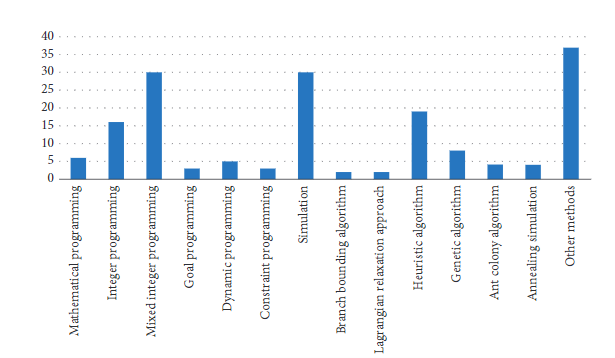
\includegraphics{Memoria TFG/img/graficoAlgoritmos.png}
    \caption{Técnicas de Optimización. Fuente \cite{Gur2018ApplicationOverview}}
    \label{GraficoTecnicasOpt}
\end{figure}

\subsection{Aproximación a la Modelización}

En función del foco a optimizar, encontramos en la literatura gran cantidad de aproximaciones a su modelización.

Podemos considerarlo como un problema de Job Shop Múltiple, o incluso como una evolución del problema de la mochila y procesamiento paralelo \cite{Lin2020AScheduling}, aunque en todos la finalidad será la misma: \textbf{asignar un bloque de tiempo, en una sala determinada, a un paciente dado} para la realización de una intervención quirúrgica.

Dependerá, por tanto, de las restricciones y los objetivos que marquemos durante la resolución, así como de la estrategia a implementar.

\subsection{Consideraciones Finales}

Como podemos comprobar, un planificación óptima de los quirófanos constituye un rol de gran importancia en los hospitales, debido a la enorme cantidad de recursos que consumen. 

A su vez, existen gran cantidad de variables a tener en cuenta, lo cual complica \cite{Lin2020AScheduling} la optimización, pudiendo llegar a incluir tantas variables (\textit{disponibilidad de cirujanos, equipamiento, anestesistas, camas hospitalarias...}) como se desee.

En nuestro caso, nos centraremos en \textbf{asignar pacientes a huecos de quirófano}, asumiendo la disponibilidad del resto de factores, debido a que la literatura se centra en la resolución de este problema y a su dificultad de implementación.

Una vez formulado el problema con nuestras restricciones, probaremos diferentes modelizaciones y algoritmos de planificación durante el transcurso del proyecto, eligiendo finalmente el que nos ofrezca mejor rendimiento de cara a la implementación final de la herramienta.